\chapter{RESULTS AND DISCUSSION}
\label{chap:evaluationresults}

\kkusection {Evaluation method}
describe evaluation method



\begin{figure}[!htbp]
\centering
\fbox{ 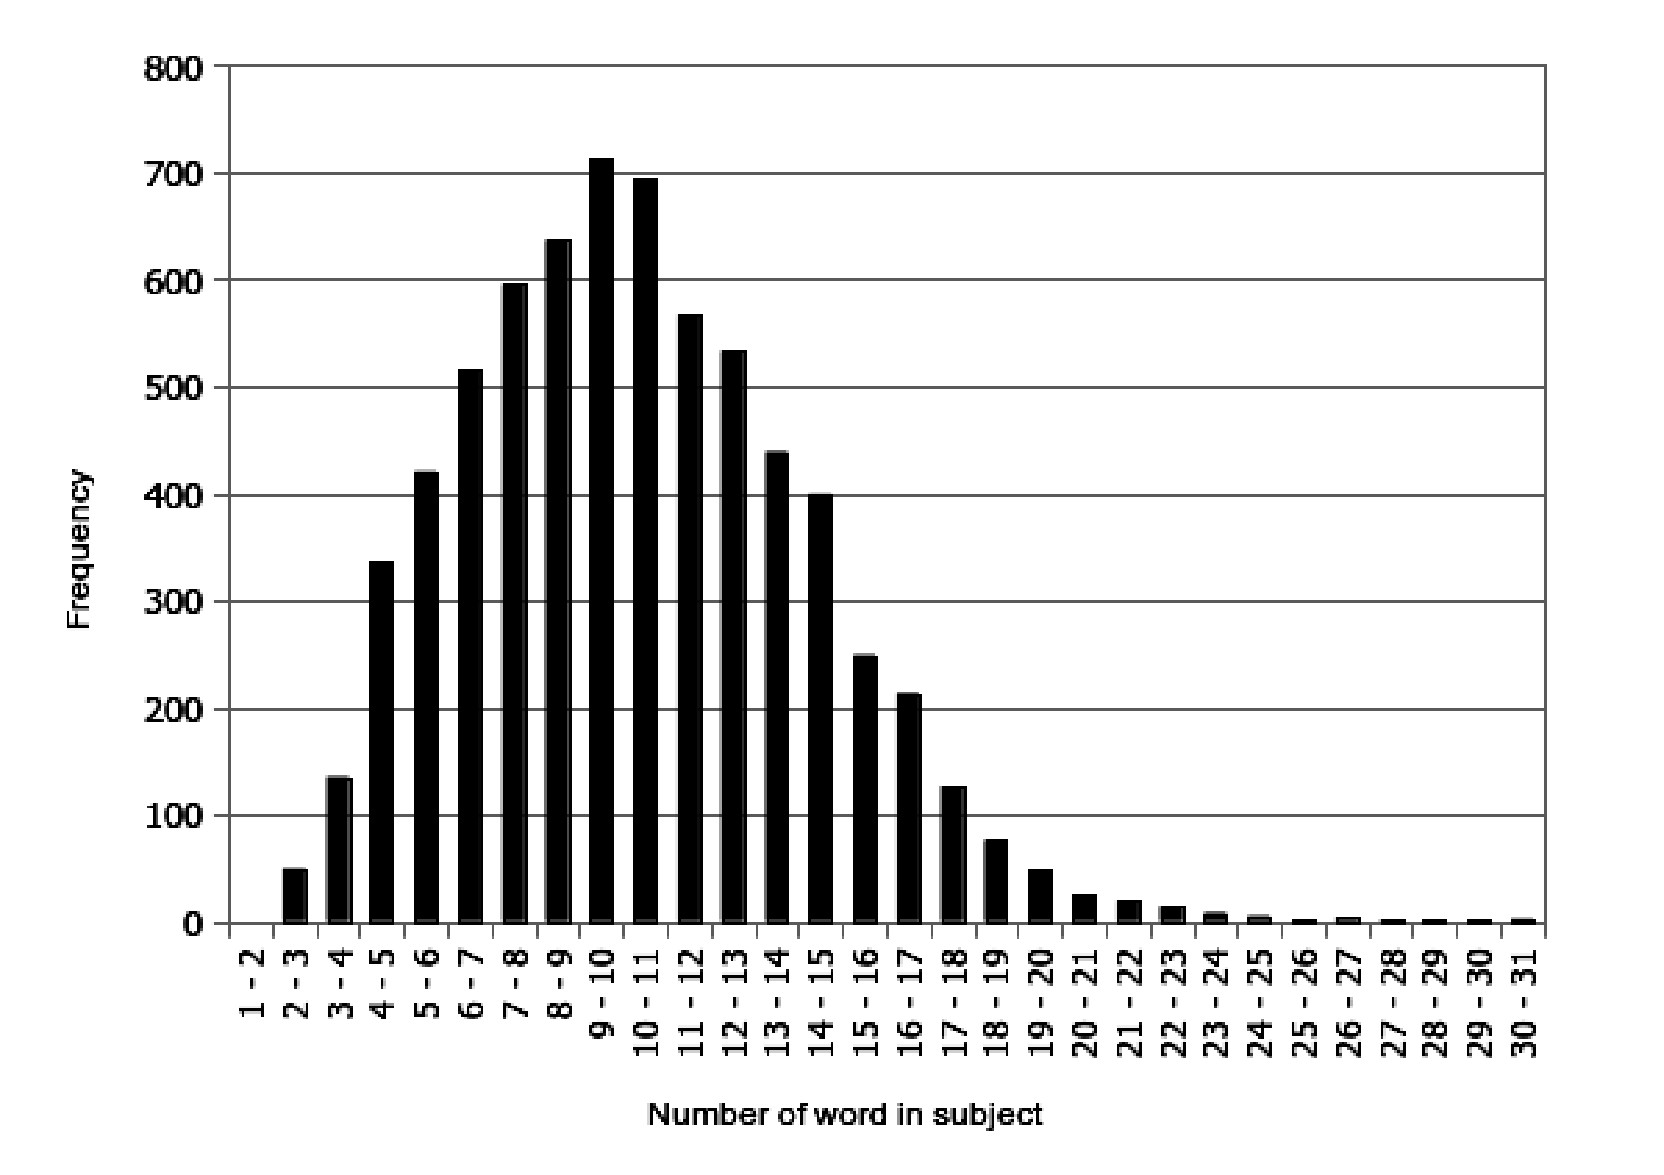
\includegraphics[scale=0.6]{./images/numberofwordsinsubject.jpg} }
\caption{Histogram for the number of words in subject in each post}
\label{figure:histogramwordinsubject}
\end{figure}


% ================================= %

\tablefirsthead{ 
\hline
\bf {Class} & \bf{Frequency} & \bf{Cumulative Frequency }\\ \hline
}

\tablehead{ 
\multicolumn{3}{ l }%
{{ \textbf{\captionsize\tablename~\thetable{}} ~ Frequency distribution table for the number of results (Cont.)}} \\
\multicolumn{3}{ l }%
{} \\
\hline
\bf {Class} & \bf{Frequency} & \bf{Cumulative Frequency }\\ 
}

\tabletail{ 
\hline
}

\tablecaption{Frequency distribution table for the number of results}

\begin{supertabular}{ | >{\centering\arraybackslash}m{1in}  | >{\centering\arraybackslash}m{1.5in}  | >{\centering\arraybackslash}m{2in}  |}

\label{tab:subjectfrequencydist}

1 - 2 & 0 & 0 \\ \hline 
2 - 3 & 49 & 49 \\ \hline 
3 - 4 & 135 & 184 \\ \hline 
4 - 5 & 336 & 520 \\ \hline 
5 - 6 & 420 & 940 \\ \hline 
6 - 7 & 515 & 1455 \\ \hline 
7 - 8 & 595 & 2050 \\ \hline 
8 - 9 & 637 & 2687 \\ \hline 
9 - 10 & 712 & 3399 \\ \hline 
10 - 11 & 694 & 4093 \\ \hline 
11 - 12 & 567 & 4660 \\ \hline 
12 - 13 & 533 & 5193 \\ \hline 
13 - 14 & 439 & 5632 \\ \hline 
14 - 15 & 399 & 6031 \\ \hline 
15 - 16 & 249 & 6280 \\ \hline 
16 - 17 & 213 & 6493 \\ \hline 
17 - 18 & 126 & 6619 \\ \hline 
18 - 19 & 76 & 6695 \\ \hline 
19 - 20 & 48 & 6743 \\ \hline 
20 - 21 & 25 & 6768 \\ \hline 
21 - 22 & 19 & 6787 \\ \hline 
22 - 23 & 14 & 6801 \\ \hline 
23 - 24 & 8 & 6809 \\ \hline 
24 - 25 & 5 & 6814 \\ \hline 
25 - 26 & 1 & 6815 \\ \hline 
26 - 27 & 3 & 6818 \\ \hline 
27 - 28 & 1 & 6819 \\ \hline 
28 - 29 & 1 & 6820 \\ \hline 
29 - 30 & 1 & 6821 \\ \hline 
30 - 31 & 2 & 6823 \\ 
\end{supertabular}


\kkusubsection { Preparing evaluation survey}


\kkusubsection { Evaluation Results }
%\clearpage
% ==================================

\kkusubsection{Satisfaction results comparison }
satisfaction

% ================================= %
\vspace{\baselineskip}
\tablefirsthead{ 
    \hline
  	& & \multicolumn{2}{ c }{\bf{System~1}} &  \multicolumn{2}{ | c }{\bf{System~2}} &  \multicolumn{2}{ | c | }{\bf{System~3}} \\
    \hline
    \bf{Question} & \bf{Type} & \bf{Mean} &  \bf{STDEV} &  \bf{Mean} &  \bf{STDEV}  &  \bf{Mean} &  \bf{STDEV}   \\ \hline
}

\tablehead{ 
\multicolumn{8}{ l }%
{{ \textbf{\captionsize\tablename~\thetable{}} ~ Comparison of satisfaction evaluation results (Cont.)}} \\
\multicolumn{8}{ l }%
{} \\
    \hline
  	& & \multicolumn{2}{ c }{\bf{System~1}} &  \multicolumn{2}{ | c }{\bf{System~2}} &  \multicolumn{2}{ | c | }{\bf{System~3}} \\
    \hline
    \bf{Question} & \bf{Type} & \bf{Mean} &  \bf{STDEV} &  \bf{Mean} &  \bf{STDEV}  &  \bf{Mean} &  \bf{STDEV}   \\  \hline
}

\tabletail{ 
\hline
}

\tablecaption{Comparison of satisfaction evaluation results}

  \begin{supertabular}{ | c | c | c | c | c | c | c | c | }  
  \label{tab:satisfactioncompare}
1 & Short & 2 &  1 & 3 & 1 & 2.33 & 1.53 \\ 
2 & Short & 1.33 &  0.58 & 3 & 1 & 2.33 & 1.53 \\ 
3 & Short & 1.33 &  0.58 & 3 & 1 & 1 & 0 \\ 
4 & Short & 1.67 &  0.58 & 3 & 0 & 2 & 1 \\ 
5 & Short & 2.33 &  1.53 & 2.67 & 1.15 & 3.67 & 1.15 \\ 
6 & Short & 1 &  0 & 2.33 & 1.53 & 1 & 0 \\ 
7 & Short & 1.33 &  0.58 & 3 & 1 & 1 & 0 \\ 
8 & Short & 2.67 &  1.15 & 3 & 1 & 1 & 0 \\ 
9 & Short & 1.67 &  1.15 & 2.33 & 0.58 & 2 & 1 \\ \hline
\bf{Average} & \bf{Short} & \bf{1.7} &  \bf{0.79} & \bf{2.81} & \bf{0.92} & \bf{1.81} & \bf{0.69} \\ \hline
10 & Medium & 2.67 &  0.58 & 3.67 & 0.58 & 1.67 & 0.58 \\ 
11 & Medium & 3 &  1 & 2.33 & 0.58 & 1.67 & 0.58 \\ 
12 & Medium & 1 &  0 & 1.33 & 0.58 & 1.33 & 0.58 \\ 
13 & Medium & 2 &  1 & 2.33 & 1.53 & 1.33 & 0.58 \\ 
14 & Medium & 1.33 &  0.58 & 3 & 0 & 3 & 1 \\ 
15 & Medium & 3 &  1 & 2.67 & 1.53 & 4 & 1.73 \\ 
16 & Medium & 1 &  0 & 3 & 1 & 2.33 & 1.53 \\ 
17 & Medium & 1.67 &  0.58 & 3 & 1 & 3.67 & 0.58 \\ 
18 & Medium & 1.33 &  0.58 & 3 & 1 & 1.67 & 0.58 \\ 
19 & Medium & 2.33 &  0.58 & 1.67 & 0.58 & 4 & 1 \\ 
20 & Medium & 2.33 &  1.15 & 2 & 0 & 1 & 0 \\ 
21 & Medium & 2.33 &  0.58 & 2.33 & 0.58 & 1.67 & 0.58 \\ 
22 & Medium & 2.33 &  1.15 & 2 & 1 & 4.67 & 0.58 \\ \hline
\bf{Average} & \bf{Medium} & \bf{2.03} &  \bf{0.67} & \bf{2.49} & \bf{0.76} & \bf{2.46} & \bf{0.76} \\ \hline
23 & Long & 1.67 &  0.58 & 2.33 & 0.58 & 3.67 & 0.58 \\ 
24 & Long & 2.67 &  0.58 & 2.67 & 0.58 & 2 & 1 \\ 
25 & Long & 2 &  1 & 3 & 1 & 3 & 0 \\ 
26 & Long & 2.33 &  0.58 & 2.67 & 0.58 & 1 & 0 \\ 
27 & Long & 1.33 &  0.58 & 3.33 & 0.58 & 2 & 1 \\ 
28 & Long & 2.33 &  1.15 & 3 & 1 & 3.67 & 0.58 \\ 
29 & Long & 1 &  0 & 3.33 & 1.15 & 1.33 & 0.58 \\ \hline
\bf{Average} & \bf{Long} & \bf{1.9} &  \bf{0.64} & \bf{2.9} & \bf{0.78} & \bf{2.38} & \bf{0.53} \\ \hline  \hline
\bf{Mean Average} &  & \bf{1.88} &  \bf{0.7} & \bf{2.74} & \bf{0.82} & \bf{2.22} & \bf{0.66} \\
  \end{supertabular}

\vspace{\baselineskip}

\begin{figure}[!htbp]
\centering
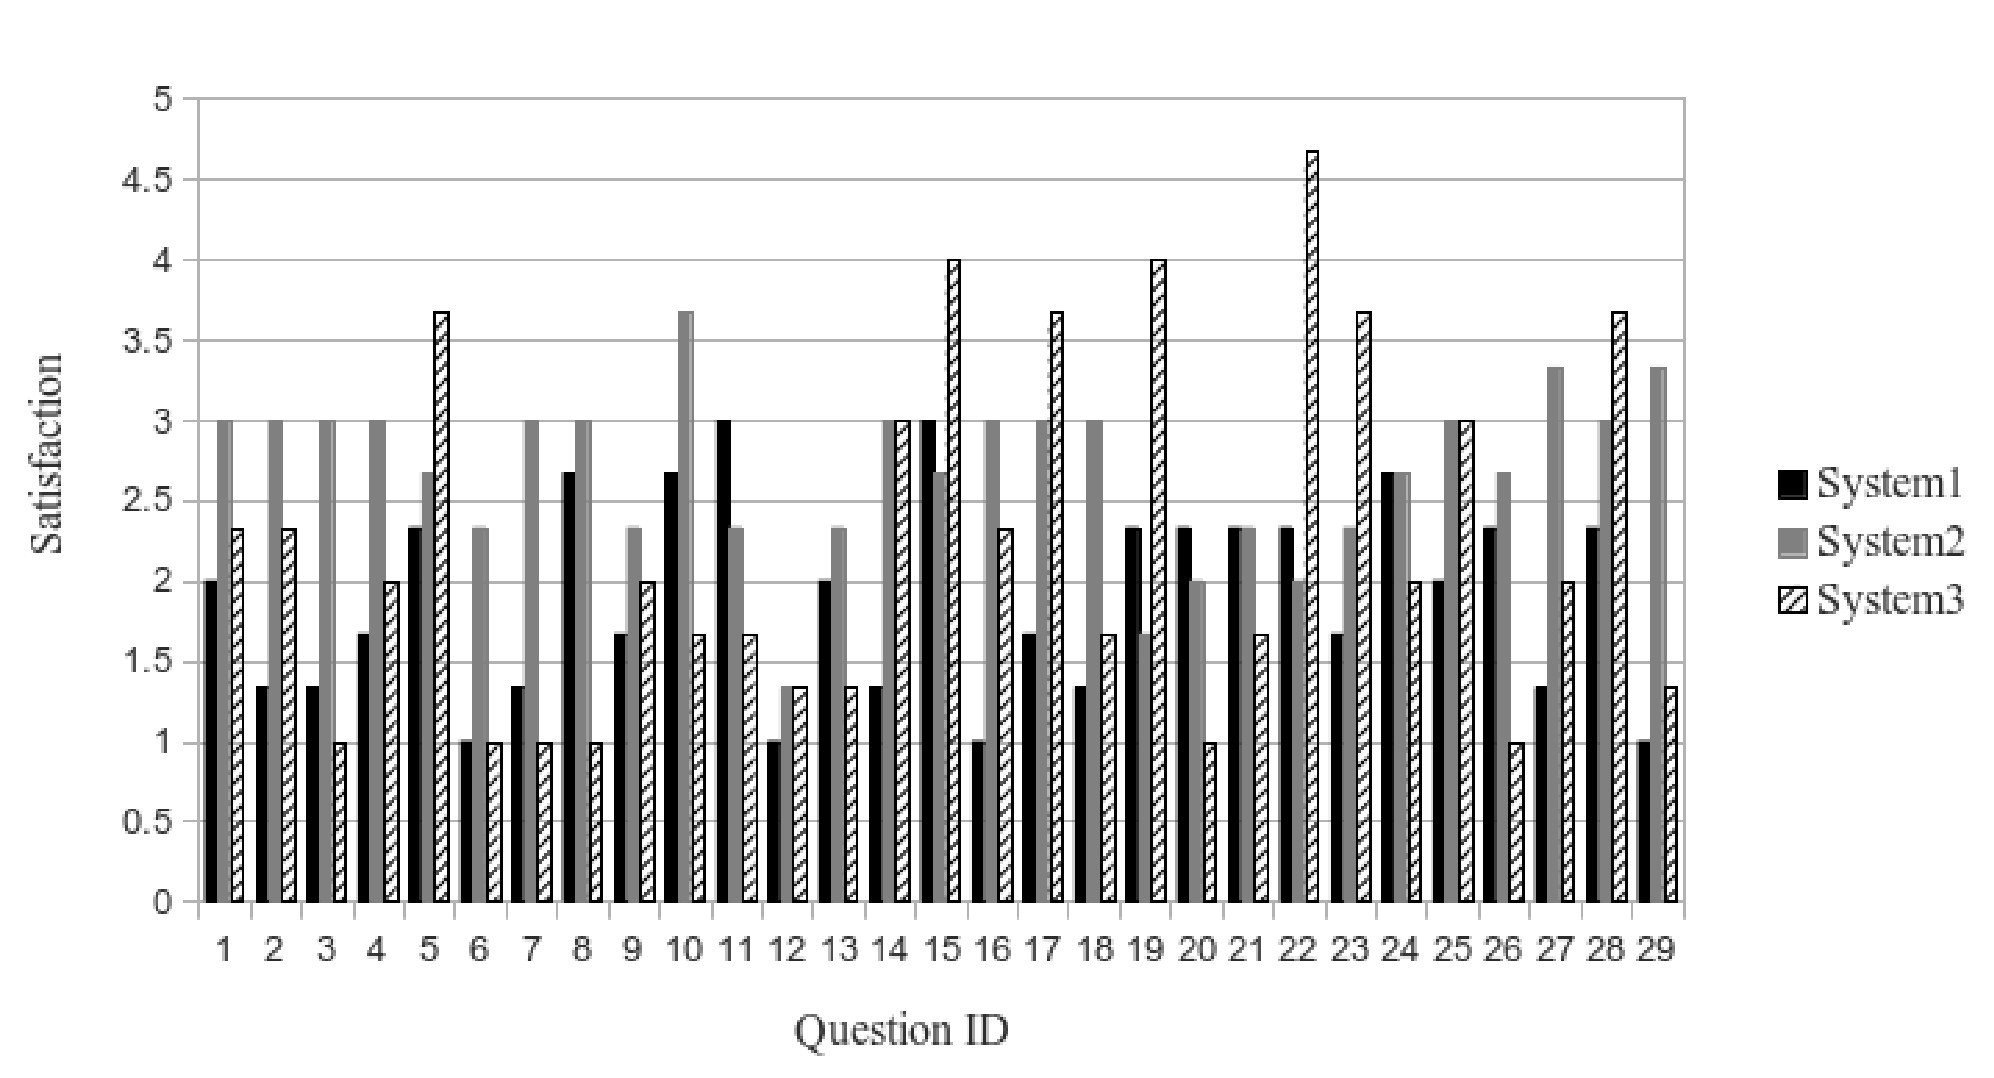
\includegraphics[scale=0.55]{./images/satisfactiongraph.jpg}
\caption{Comparison graph of satisfaction evaluation results}
\label{figure:satisfactiongraph}
\end{figure}

